\documentclass[12pt,twoside]{book}

\usepackage[utf8]{inputenc}
\usepackage[turkish]{babel}
\usepackage[T1]{fontenc}

\usepackage{amsmath}
\usepackage{amssymb}
\usepackage{amsthm}
\usepackage{enumerate}
\usepackage[most]{tcolorbox}

\usepackage{circuitikz}
\usepackage{cancel}
\usepackage{bodegraph}
\usepackage{gensymb}

\usepackage{verbatim}
\usepackage{listings}
\usepackage{matlab-prettifier}

\usepackage{pgfplots}
\pgfplotsset{compat=newest}
\usepackage{pgffor}
\usepackage{xcolor}

\usepackage{tikz}
\usetikzlibrary{patterns}
\usetikzlibrary{babel}

\usetikzlibrary{shapes.misc}
\tikzset{cross/.style={cross out, draw=black, minimum size=2*(#1-\pgflinewidth), inner sep=0pt, outer sep=0pt},
%default radius will be 3pt. 
cross/.default={3pt}}
\usetikzlibrary{arrows}
\tikzset{
  arrow/.pic={\path[tips,every arrow/.try,->,>=#1] (0,0) -- +(.1pt,0);},
  pics/arrow/.default={triangle 90}
}

\usepackage{siunitx}
\usepackage{textcomp}

\usepackage{hyperref}
\hypersetup{
    colorlinks=true,
    linkcolor=blue,
    filecolor=magenta,      
    urlcolor=cyan,
    pdftitle={Kitap},
    pdfpagemode=FullScreen,
    }

\urlstyle{same}

\usepackage{graphicx}
\graphicspath{{svg-inkscape/}}
\usepackage{geometry}
\usepackage{subcaption}
\usepackage{tabularray}
\usepackage{tabularx}
\DefTblrTemplate{contfoot-text}{default}{Bir sonraki sayfada devam ediyor.} % Uzun Tablolar için alt kısım
\DefTblrTemplate{conthead-text}{default}{(Devam)} % Uzun Tablolar için üst kısım

\usepackage{lscape}

\usepackage{pgfplotstable}
\usepackage{booktabs}

\renewcommand{\chaptername}{Bölüm}
\renewcommand{\contentsname}{İçindekiler}
\renewcommand{\figurename}{Şekil}
\renewcommand{\tablename}{Tablo}
\renewcommand{\bibname}{Kaynaklar}
\renewcommand{\listfigurename}{Şekiller}
\renewcommand{\listtablename}{Tablolar}
\renewcommand{\appendixname}{Ek}
\renewcommand{\indexname}{Dizin}
\renewcommand{\partname}{Bölüm}
\renewcommand{\proofname}{İspat}

\begin{document}
\shorthandoff{=} % babel paketi hatasını gidermek için gerekli

\tableofcontents

\documentclass[12pt,hyperref=unicode]{beamer}

\usepackage[utf8]{inputenc}
\usepackage[turkish]{babel}
\usepackage[T1]{fontenc}

\usepackage{amsmath}
\usepackage{amssymb}
\usepackage{amsthm}
\usepackage{enumerate}
\usepackage{tikz}
\usepackage{transparent}
\usepackage{xcolor}
\usepackage{listings}
\usepackage{verbatim}
\usepackage{graphicx}

\usepackage{pgfplots}

\usetheme{Warsaw}
\usecolortheme{default}
\definecolor{nigdeyesili_acik}{RGB}{3, 150, 166}
\definecolor{nigdeyesili_koyu}{RGB}{143, 209, 217}
\setbeamercolor{structure}{fg=nigdeyesili_acik}

\author[Dr. Mehmet CANEVİ]{Arş.~Gör.~Dr.~M.~Canevi\inst{1}}

\institute{
    \inst{1}%
    Bilgisayar Mühendisliği\\
    Mühendislik Fakültesi
}
    
\date[2025] {Ders Notları, Ocak 2025}
\setbeamertemplate{footline}[frame number]

\logo{\transparent{0.4}
\includegraphics[width = 20mm]{logo}}

\definecolor{mGreen}{rgb}{0,0.6,0}
\definecolor{mGray}{rgb}{0.5,0.5,0.5}
\definecolor{mPurple}{rgb}{0.58,0,0.82}
\definecolor{backgroundColour}{rgb}{0.95,0.95,0.92}

\lstloadlanguages{C}
\lstdefinestyle{CStyle}{
    backgroundcolor=\color{backgroundColour},   
    commentstyle=\color{mGreen},
    keywordstyle=\color{red},
    numberstyle=\tiny\color{mGray},
    stringstyle=\color{mGreen},
    basicstyle=\footnotesize,
    breakatwhitespace=false,         
    breaklines=true,                 
    captionpos=b,                    
    keepspaces=true,                 
    numbers=left,                    
    numbersep=2pt,                  
    showspaces=false,                
    showstringspaces=false,
    showtabs=false,                  
    tabsize=1,
    language=C
}
\lstset{style=CStyle}

\AtBeginDocument{\shorthandoff{=}}
\title[Ders 1] {Kod Yazma, Kod Derleme. Değişken Tanımlama, Veri Tipleri. Operatörler.}
\begin{document}
%%%%%%%%%%%%%%%%%%%%%%%%%%%%%%%%%%%%%%%%%%%%%%%%%%%%%%%%%%%%%%%%%%%%%%%%%%%%%%%%
\frame{\titlepage}
\begin{frame}[fragile]{İçidekiler}
    \tableofcontents
\end{frame}
%%%%%%%%%%%%%%%%%%%%%%%%%%%%%%%%%%%%%%%%%%%%%%%%%%%%%%%%%%%%%%%%%%%%%%%%%%%%%%%%
\section{Kod yazma}
\begin{frame}[fragile]{Kod nedir?}
    \begin{itemize}
        \item Bilgisayar tanımı kapsamına giren cihazlara meramımızı anlatmak için yazılan yazıya \textbf{kod} diyebiliriz
        \item Bahsi geçen yazının bir dili olur ve buna kodun dili denir
        \item Bu ders kapsamında \verb|C| dilini kullanacağız
        \item \verb|C| dili insanın anlama şekline daha yakındır
        \item Makinenin anlama şekline yakın diline \textbf{makine dili} denir
    \end{itemize}
\end{frame}
%%%%%%%%%%%%%%%%%%%%%%%%%%%%%%%%%%%%%%%%%%%%%%%%%%%%%%%%%%%%%%%%%%%%%%%%%%%%%%%%
\begin{frame}[fragile]{Derleme nedir?}
    \begin{itemize}
        \item \verb|C| dilinden \textbf{makine dili}ne çeviri işlemidir
        \item Kod yazarken yapılan her güncelleme sonrası derlemeye ihtiyaç duyulur
        \item Derleme bazen hata ile sonuçlanabilir, muhtemel bir \textbf{imla hatası} sebep olabilir
        \item Derleme başarılı olmasına rağmen makine istenen davranışı göstermeyebilir(\textbf{mantıksal hata})
        \item \verb|Windows| için derleme(ve linkleme sonucu) \verb|exe| uzantılı bir dosya üretilir
    \end{itemize}
\end{frame}
%%%%%%%%%%%%%%%%%%%%%%%%%%%%%%%%%%%%%%%%%%%%%%%%%%%%%%%%%%%%%%%%%%%%%%%%%%%%%%%%
\begin{frame}[fragile]{Örnek bir kod}
    Örnek bir kod
    \lstinputlisting{lec1/main.c}
    şeklindedir.
\end{frame}
%%%%%%%%%%%%%%%%%%%%%%%%%%%%%%%%%%%%%%%%%%%%%%%%%%%%%%%%%%%%%%%%%%%%%%%%%%%%%%%%
\begin{frame}[fragile]{Örnek bir makine kodu}
    Örnek bir makine kodu
    \lstinputlisting{lec1/main.o}
    şeklindedir.
\end{frame}
%%%%%%%%%%%%%%%%%%%%%%%%%%%%%%%%%%%%%%%%%%%%%%%%%%%%%%%%%%%%%%%%%%%%%%%%%%%%%%%%
\begin{frame}[fragile]{Makine kodunun temeli}
    $4+6$ işlemini inceleyelim:
    \begin{equation}
        (0100)_2+(0110)_2=(1010)_2=10
    \end{equation}
    1 bitlik en basit toplama işlemi 
    \begin{figure}[!htb]
        \centering
        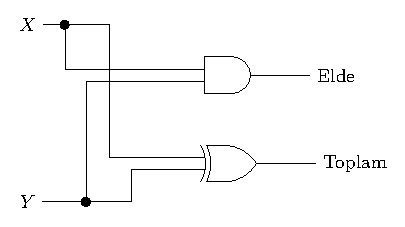
\includegraphics[width=0.5\textwidth]{lec1/xor}
    \end{figure}
    ile gösterilebilir. 4 bit için bu yapı temel alınıp gerçeklenebilir.
\end{frame}
%%%%%%%%%%%%%%%%%%%%%%%%%%%%%%%%%%%%%%%%%%%%%%%%%%%%%%%%%%%%%%%%%%%%%%%%%%%%%%%%
\begin{frame}[fragile]{Makine kodunun temeli(devam)}
    4 bit için bu yapı 
    \begin{figure}[!htb]
        \centering
        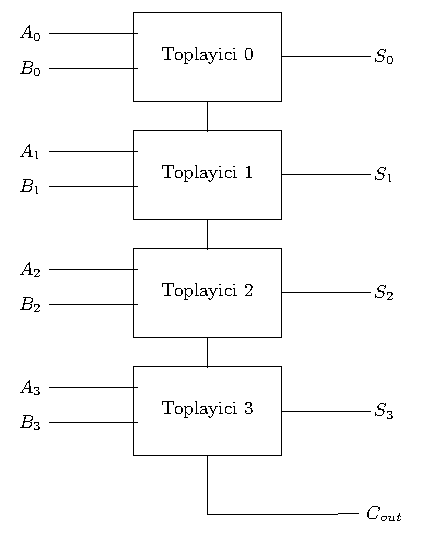
\includegraphics[height=0.6\textheight]{lec1/fulladder}
    \end{figure}
    şeklinde gösterilebilir.
\end{frame}
%%%%%%%%%%%%%%%%%%%%%%%%%%%%%%%%%%%%%%%%%%%%%%%%%%%%%%%%%%%%%%%%%%%%%%%%%%%%%%%%
\begin{frame}[fragile]{Makine kodunun temeli(devam)}
    \begin{itemize}
    \item 4 bitlik toplama devresi \textbf{çıkarma işlemi}, \textbf{çarpma işlemi} vb. işlemler ile aritmetik işlemci oluşturulabilmektedir. 
    \item Mantıksal işlemler için de tasarlanırsa ortaya Aritmetik Lojik Birim(ALB) ortaya çıkmaktadır. 
    \item Merkezi İşlemci Birimi(MİB) denilen karmaşık yapının başlangıcı denebilir.
    \end{itemize}
\end{frame}
%%%%%%%%%%%%%%%%%%%%%%%%%%%%%%%%%%%%%%%%%%%%%%%%%%%%%%%%%%%%%%%%%%%%%%%%%%%%%%%%
\section{Değişken tanımlama ve veri tipleri}
\begin{frame}[fragile]{Değişken isimleri}
    Değişkenler şu şekilde tanımlanmaktadır:
    \begin{lstlisting}
        veri_tipi degisken_adi;
        veri_tipi degisken_adi=ilk_deger;\end{lstlisting}
    Buradaki \lstinline{veri_tipi};
    \begin{itemize}
        \item \lstinline{int} 
        \item \lstinline{float}
        \item \lstinline{double}
        \item \lstinline{char}
    \end{itemize}
     olabilmektedir. \lstinline{degisken_adi} ise 
    \begin{itemize}
     \item türkçe karakter içermemelidir
     \item sadece harf veya alttire ile başlamalıdır
     \item özel karakterler(!,?,vb.) ve boşluk içermemelidir
     \item \lstinline{veri_tipi} anahtar kelimeleri olmamalıdır
    \end{itemize}
    kurallarına uymalıdır.
\end{frame}
%%%%%%%%%%%%%%%%%%%%%%%%%%%%%%%%%%%%%%%%%%%%%%%%%%%%%%%%%%%%%%%%%%%%%%%%%%%%%%%%
\begin{frame}[fragile]{Değişken tiplerinin anlamı}
    Değişkenler
    \begin{itemize}
     \item \lstinline{int} ingilizce \verb|integer| yani tam sayıdan gelmektedir \lstinline{-10,4} gibi
     \item \lstinline{float} ingilizcede kayan noktalı sayı(6-7 basamak) anlamındadır \lstinline{3.14f} gibi
     \item \lstinline{double} ingilizcede iki kat hassasiyet(15 basamak) anlamındadır \lstinline{3.14} gibi
     \item \lstinline{char} ingilizce \verb|character|'den gelir \lstinline{'c','x'} gibi
    \end{itemize}
    veri tipleri ile tanımlanabilmektedir ve 
    \begin{itemize}
        \item \lstinline{int var1=-10;} 
        \item \lstinline{float var2=3.14f;} 
        \item \lstinline{double var3=3.14;} 
        \item \lstinline{char var4='x';} 
    \end{itemize}
    olarak örneklendirilebilir.
\end{frame}
%%%%%%%%%%%%%%%%%%%%%%%%%%%%%%%%%%%%%%%%%%%%%%%%%%%%%%%%%%%%%%%%%%%%%%%%%%%%%%%%
\begin{frame}[fragile]{Çoklu değişken tanımlama}
    Birden fazla değişken
    \begin{itemize}
        \item \lstinline{int a,b,c=-10;} 
        \item \lstinline{float a=2.2,b,c=3.14f;} 
        \item \lstinline{double a,b,c=3.14;} 
        \item \lstinline{char a,b,c;a=b=c='x';}
    \end{itemize}
    şeklinde tanımlanabilir.
\end{frame}
%%%%%%%%%%%%%%%%%%%%%%%%%%%%%%%%%%%%%%%%%%%%%%%%%%%%%%%%%%%%%%%%%%%%%%%%%%%%%%%%
\begin{frame}[fragile]{Değişkenlerin yazdırılması}
    Değişkenler
    \begin{itemize}
        \item \lstinline{int var1=-10;printf("%d",var1);} 
        \item \lstinline{float var2=3.14f;printf("%f",var2);} 
        \item \lstinline{double var3=3.14;printf("%lf",var3);} 
        \item \lstinline{char var4='x';printf("%c",var4);}
        \item \lstinline{printf("%s","Bu bir cumledir.");}
    \end{itemize}
    ile ekrana yazdırılır.
\end{frame}
%%%%%%%%%%%%%%%%%%%%%%%%%%%%%%%%%%%%%%%%%%%%%%%%%%%%%%%%%%%%%%%%%%%%%%%%%%%%%%%%
\begin{frame}[fragile]{Sabit değerli değişkenler}
    Değeri değişmemesi gereken değişkenler
    \begin{itemize}
        \item \lstinline{const int SAAT_DK=60;} 
        \item \lstinline{const float PI_SAYISI=3.14;} 
    \end{itemize}
    şeklinde tanımlanır ve büyük harflerin kullanımı bir gelenektir. Dolayısıyla,
    \begin{itemize}
        \item \lstinline{SAAT_DK=120;} 
        \item \lstinline{PI_SAYISI=5.5;} 
    \end{itemize}
    hata verir.
\end{frame}
%%%%%%%%%%%%%%%%%%%%%%%%%%%%%%%%%%%%%%%%%%%%%%%%%%%%%%%%%%%%%%%%%%%%%%%%%%%%%%%%
\section{Operatörler}
\begin{frame}[fragile]{Matematiksel operatörler}
    Toplama ve çıkarma işlemi
    \begin{itemize}
        \item \lstinline{int a=4+5;int c=a-2;int d=a+c;} 
    \end{itemize}
    ile örneklendirilebilir. Matematiksel operatörler
    \begin{itemize}
        \item \lstinline{+,-} toplama, çıkarma 
        \item \lstinline{*,/} çarpma, bölme
        \item \lstinline{++,--} arttırma, azaltma 
        \item \lstinline{%} \verb|mod| operatörü (bölümden kalan)
        \item \lstinline{=} atama operatörü
    \end{itemize}
    şeklindedir.
\end{frame}
%%%%%%%%%%%%%%%%%%%%%%%%%%%%%%%%%%%%%%%%%%%%%%%%%%%%%%%%%%%%%%%%%%%%%%%%%%%%%%%%
\begin{frame}[fragile]{Matematiksel operatörler(devam)}
    Aşağıdaki operatörler tanımlıdır.
    \begin{itemize}
        \item \lstinline{x+=3;} \lstinline{x=x+3;} 
        \item \lstinline{x-=3;} \lstinline{x=x-3;} 
        \item \lstinline{x*=3;} \lstinline{x=x*3;} 
        \item \lstinline{x/=3;} \lstinline{x=x/3;} 
        \item \lstinline{x%=3;} \lstinline{x=x%3;} 
    \end{itemize}
\end{frame}
%%%%%%%%%%%%%%%%%%%%%%%%%%%%%%%%%%%%%%%%%%%%%%%%%%%%%%%%%%%%%%%%%%%%%%%%%%%%%%%%
\begin{frame}[fragile]{Karşılaştırma operatörleri}
    Aşağıdaki operatörler ile karşılaştırma başarılı ise 1 değilse sıfır değerini alır.
    \begin{itemize}
        \item \lstinline{x>y} Büyüktür
        \item \lstinline{x>=y} Büyük eşittir
        \item \lstinline{x<y} Küçüktür
        \item \lstinline{x<=y} Küçük eşittir
        \item \lstinline{x==y} Eşittir
        \item \lstinline{x!=y} Eşit değildir
    \end{itemize}
\end{frame}
%%%%%%%%%%%%%%%%%%%%%%%%%%%%%%%%%%%%%%%%%%%%%%%%%%%%%%%%%%%%%%%%%%%%%%%%%%%%%%%%
\begin{frame}[fragile]{Mantıksal operatörleri}
    Mantıksal operatörler
    \begin{itemize}
        \item \lstinline{sart1 && sart2} VE
        \item \lstinline{sart1 || sart2} VEYA 
        \item \lstinline{!sart} DEĞİLDİR 
    \end{itemize}
    olarak verilmiştir.
\end{frame}
%%%%%%%%%%%%%%%%%%%%%%%%%%%%%%%%%%%%%%%%%%%%%%%%%%%%%%%%%%%%%%%%%%%%%%%%%%%%%%%%
\end{document}

\end{document}
